% -------------------- 第 1 章:参赛作品使用的AI工具列表 --------------------
\section{参赛作品使用的AI工具列表}

\begin{itemize}
    \item \textbf{ChatGPT:} GPT, o4, OpenAI, 2025-09-05
    \item \textbf{Kimi:} Kimi, Latest, 月之暗面, 2025-09-05
    \item \textbf{DeepSeek:}  DeepSeek, R1 0528, 深度求索(DeepSeek), 2025-09-05
    \item \textbf{Github Copilot:} Github Copilot, GitHub, 2025-09-05
    \item \textbf{Qwen:} Qwen, 320B, 2025-09-05
    \item \textbf{Claude:} Claude, 4.0 Sonnet, Anthropic, 2025-09-05
    \item \textbf{Gemini:} Gemini, 1.5 Pro, Google DeepMind, 2025-09-05
\end{itemize}

% 根据列表建立环境
% ChatGPT Block
\newenvironment{GPTblock}
{
    \begin{block}[colback=blue!5, colframe=blue!50, title={
        \raisebox{-.2em}{
\includegraphics[height=1.5em]{icons/openai.png}}\hspace{0.5em}\textcolor{black}{ChatGPT}
    }]
}
{
    \vspace{0.5em}
    \begin{flushright}
        \scriptsize
        \textbf{模型使用信息:} ChatGPT,GPT,o4,OpenAI,2025-09-05
    \end{flushright}
    \end{block}
}

% Kimi Block
\newenvironment{KimiBlock}
{
    \begin{block}[colback=purple!5, colframe=purple!50, title={
        \raisebox{-.2em}{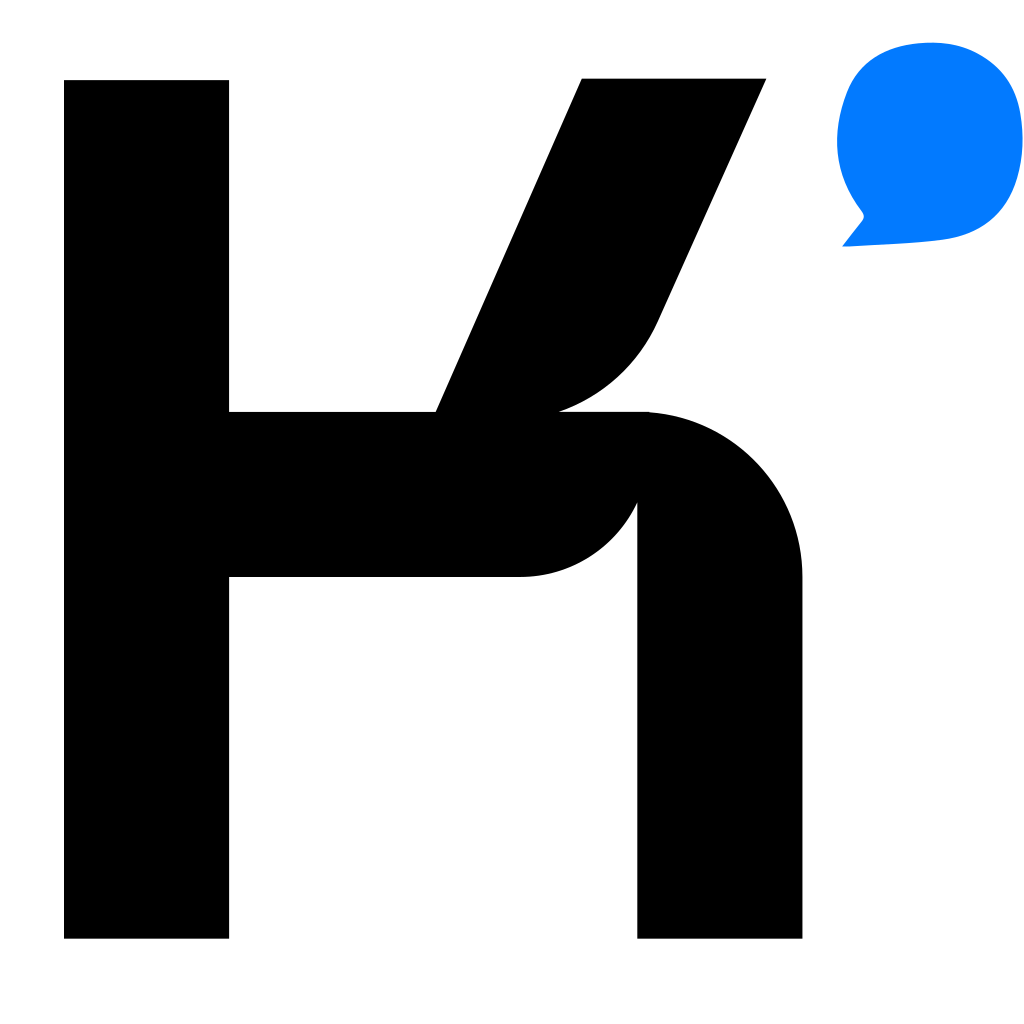
\includegraphics[height=1.5em]{icons/kimi-color.png}}\hspace{0.5em}\textcolor{black}{Kimi}
    }]
}
{
    \vspace{0.5em}
    \begin{flushright}
        \scriptsize
        \textbf{模型使用信息:} Kimi,Latest,月之暗面,2025-09-05
    \end{flushright}
    \end{block}
}

% DeepSeek Block
\newenvironment{DeepSeekBlock}
{
    \begin{block}[colback=cyan!5, colframe=cyan!50, title={
        \raisebox{-.2em}{
\includegraphics[height=1.5em]{icons/deepseek-color.png}}\hspace{0.5em}\textcolor{black}{DeepSeek}
    }]
}
{
    \vspace{0.5em}
    \begin{flushright}
        \scriptsize
        \textbf{模型使用信息:} DeepSeek,R1 0528,深度求索(DeepSeek),2025-09-05
    \end{flushright}
    \end{block}
}

% Copilot Block
\newenvironment{CopilotBlock}
{
    \begin{block}[colback=gray!5, colframe=gray!50, title={
        \raisebox{-.2em}{
\includegraphics[height=1.5em]{icons/githubcopilot.png}}\hspace{0.5em}\textcolor{black}{Github Copilot}
    }]
}
{
    \vspace{0.5em}
    \begin{flushright}
        \scriptsize
        \textbf{模型使用信息:} Github Copilot,GitHub,2025-09-05
    \end{flushright}
    \end{block}
}

% Qwen Block
\newenvironment{QwenBlock}
{
    \begin{block}[colback=yellow!5, colframe=yellow!50, title={
        \raisebox{-.2em}{
\includegraphics[height=1.5em]{icons/qwen-color.png}}\hspace{0.5em}\textcolor{black}{Qwen}
    }]
}
{
    \vspace{0.5em}
    \begin{flushright}
        \scriptsize
        \textbf{模型使用信息:} Qwen,320B,2025-09-05
    \end{flushright}
    \end{block}
}

% Claude Block
\newenvironment{ClaudeBlock}
{
    \begin{block}[colback=orange!5, colframe=orange!50, title={
        \raisebox{-.2em}{
\includegraphics[height=1.5em]{icons/claude-color.png}}\hspace{0.5em}\textcolor{black}{Claude}
    }]
}
{
    \vspace{0.5em}
    \begin{flushright}
        \scriptsize
        \textbf{模型使用信息:} Claude,4.0 Sonnet,Anthropic,2025-09-05
    \end{flushright}
    \end{block}
}

% Gemini Block
\newenvironment{GeminiBlock}
{
    \begin{block}[colback=teal!5, colframe=teal!50, title={
        \raisebox{-.2em}{
\includegraphics[height=1.5em]{icons/gemini-color.png}}\hspace{0.5em}\textcolor{black}{Gemini}
    }]
}
{
    \vspace{0.5em}
    \begin{flushright}
        \scriptsize
        \textbf{模型使用信息:} Gemini,1.5 Pro,Google DeepMind,2025-09-05
    \end{flushright}
    \end{block}
}

